\section{What is Computation?}

The classical theory of computation, developed through pioneering work on effective procedures and mechanical calculation, established computation as the manipulation of discrete symbols according to formal rules \cite{Turing1936}. However, ECC suggests that consciousness requires a fundamentally different kind of computation—one grounded in continuous, physically embodied energy flows rather than abstract symbol manipulation \cite{MacLennan2004}.

Traditional computational theory centers on the notion that any computation can be reduced to a sequence of simple, mechanical steps executed by an abstract machine \cite{Copeland2017}. The universal Turing machine demonstrated that all classical computation could be realized through the manipulation of discrete symbols on an infinite tape. The Church-Turing thesis suggested that any intuitively computable function could be computed by these equivalent formalisms, establishing a foundational principle for computer science \cite{Smith2002}.

However, these classical approaches share crucial assumptions that ECC challenges. First, they presume that information can be perfectly encoded in discrete states, while ECC argues that conscious processing requires continuous, analog-like states that cannot be \textbf{fully} captured by discrete representations \cite{vanGelder1995}. Second, the Church-Turing thesis implies that computation is independent of its physical implementation, whereas ECC contends that consciousness requires specific physical properties and energy dynamics that cannot be abstracted away \cite{Landauer1996}.

These theoretical tensions highlight fundamental questions about the nature of computation itself. While the Church-Turing thesis may capture the essence of abstract symbol manipulation, consciousness appears to require what \cite{Piccinini2015} terms natural computation—physically embodied processes that cannot be reduced to discrete symbolic operations. This suggests that understanding consciousness requires expanding our conception of computation beyond traditional algorithmic frameworks.

\begin{figure}[h]
    \centering
    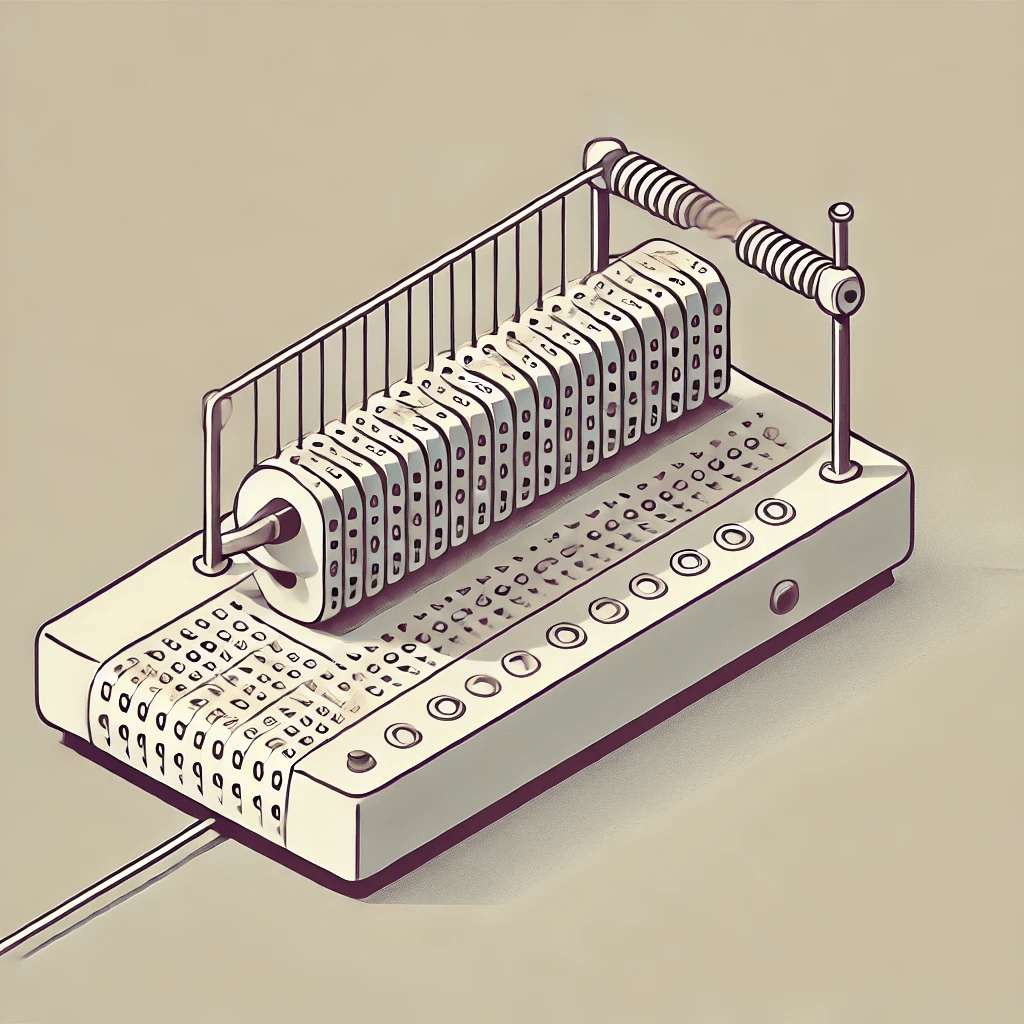
\includegraphics[width=0.8\textwidth]{turing.png}

    \caption{Artwork depicting a simple realization of an abstract Turing machine}
\end{figure}

The relationship between physical implementation and computation takes on particular significance in ECC's framework. While traditional computational theory treats physical substrates as incidental to computational processes \cite{Chalmers2011}, ECC suggests that certain physical properties—particularly those enabling coherent energy flows—are essential to conscious computation \cite{Landauer1996}. This perspective aligns with emerging understanding of how biological systems process information through continuous, physically grounded dynamics rather than discrete state transitions.

Recent theoretical work has begun to challenge the assumption that all natural processes admit computational description \cite{Searle1990}. Just as digestion cannot be adequately characterized as information processing, and gravitational phenomena cannot be reduced to computation, conscious experience may emerge from physical dynamics that resist computational abstraction \cite{vanGelder1995}. This aligns with growing skepticism about the computational theory of mind, particularly regarding the context-sensitivity and holistic nature of conscious thought.

TODO: G Ryle cite on category error below?

The framework suggests that attempting to reduce consciousness to computation represents what \cite{Smith2002} identifies as a category error—confusing the abstract map of computational description with the physical territory of conscious experience. While computational models may capture certain aspects of cognitive processing, they fundamentally miss the continuous, field-like properties that characterize conscious experience \cite{Piccinini2015}. This limitation becomes particularly evident when considering how consciousness maintains coherence across distributed neural processes.

Traditional computationalism faces particular challenges in explaining the temporal dynamics of consciousness \cite{Siegelmann2003}. The continuous flow of conscious experience appears fundamentally at odds with the discrete state transitions that characterize classical computation. ECC suggests that this temporal continuity emerges naturally from the physical dynamics of coherent energy flows, rather than requiring additional computational mechanisms to bridge discrete states.

The implications extend beyond theoretical understanding to practical questions about artificial consciousness \cite{Aaronson2013}. While digital computers excel at manipulating discrete symbols according to formal rules, they may be fundamentally incapable of supporting the specific forms of energetic coherence that ECC identifies as essential to conscious experience. This suggests that creating conscious artificial systems might require radically different approaches to computation and physical implementation.

The distinction between classical computation and conscious processing becomes particularly evident when examining how biological systems maintain coherent states across multiple scales \cite{MacLennan2004}. Unlike digital computers that maintain sharp boundaries between processing elements, conscious systems operate through continuous fields of influence that span multiple levels of organization. The resulting integration cannot be achieved through discrete computational steps but requires physical processes that maintain coherence through direct energetic interaction.

This perspective suggests a fundamental revision of how we understand computation in biological systems \cite{Adriaans2013}. Rather than viewing neural computation as analogous to digital processing, ECC proposes that conscious systems compute through patterns of energetic coherence that enable both stability and flexibility. This aligns with emerging views in theoretical neuroscience that emphasize the importance of continuous, dynamical processes in neural computation \cite{Piccinini2015}.

Recent work has begun to formalize these distinctions through mathematical frameworks that capture the continuous, field-like properties of conscious processing \cite{Siegelmann2003}. These approaches suggest that conscious computation operates in a fundamentally different regime from classical digital computation, one characterized by coherent energy flows rather than discrete state transitions. This mathematical perspective helps explain why consciousness exhibits properties that appear difficult or impossible to replicate through traditional computational approaches.

The relationship between energy and information takes on particular significance in this context \cite{Landauer1996}. While classical computation treats information as abstract and substrate-independent, ECC suggests that conscious processing requires specific physical implementations that enable particular patterns of energy flow and transformation. This perspective aligns with fundamental insights about the physical nature of information while suggesting new approaches to understanding how conscious systems process and integrate information.

The framework also provides insight into why certain aspects of conscious experience appear resistant to computational modeling \cite{Searle1990}. Features such as qualitative experience, temporal continuity, and global integration may emerge naturally from the physical dynamics of conscious systems while remaining fundamentally irreducible to discrete computational processes. This suggests that understanding consciousness requires moving beyond purely computational approaches to consider the physical basis of conscious experience.

This reconceptualization of computation through ECC's framework raises fundamental questions about the nature of conscious processing \cite{Wheeler1990}. While traditional approaches treat consciousness as emerging from abstract information processing, ECC suggests that conscious experience requires specific forms of physical organization that enable coherent energy dynamics. This perspective helps explain both the remarkable capabilities of conscious systems and their fundamental limitations.

The relationship between computation and physical implementation becomes particularly significant when considering the temporal aspects of conscious processing \cite{Deutsch2011}. Unlike classical computation, which proceeds through discrete time steps, consciousness exhibits continuous temporal evolution that emerges from the physical dynamics of neural systems. This temporal continuity appears essential to conscious experience yet proves difficult or impossible to capture through traditional computational frameworks.

Recent theoretical work has begun to explore how physical constraints shape the computational capabilities of conscious systems \cite{Fodor1981}. Rather than viewing these constraints as limitations to be overcome, ECC suggests they play a constructive role in enabling the specific forms of computation necessary for consciousness. This perspective aligns with emerging understanding of how biological systems achieve sophisticated information processing through their physical organization \cite{Smith2002}.

The framework provides particular insight into the relationship between local and global aspects of conscious computation \cite{vanGelder1995}. While traditional computational approaches often struggle to explain how distributed processing gives rise to unified experience, ECC suggests that this integration emerges naturally from the physical dynamics of coherent energy flows. This helps explain how consciousness achieves both differentiated processing and global coherence without requiring additional computational mechanisms.

These theoretical insights have important implications for understanding both biological consciousness and artificial systems \cite{Piccinini2015}. While digital computers may excel at certain forms of information processing, they appear fundamentally limited in their ability to support the specific types of computation that ECC identifies as essential to consciousness. This suggests that creating conscious artificial systems might require radically different approaches to computation and physical implementation.

The distinction between classical and conscious computation illuminates fundamental questions about the nature of mind and experience \cite{Chalmers2011}. ECC suggests that consciousness represents a unique form of physical computation that cannot be reduced to abstract symbol manipulation or discrete state transitions. This perspective helps resolve longstanding debates about the relationship between computation and consciousness while suggesting new directions for research and development.

The apparent tension between ECC's non-computational account of consciousness and its retention of "computation" in its name resolves through careful consideration of how the framework redefines computation itself \cite{MacLennan2004}. Rather than rejecting computation entirely, ECC reconceptualizes it as emerging from physical dynamics that maintain specific patterns of energetic coherence. This broadened understanding of computation aligns with recent theoretical work suggesting that biological systems compute through continuous, physically-grounded processes rather than discrete symbolic operations \cite{Siegelmann2003}. ECC accepts that consciousness implies computation but not vice versa.

This theoretical synthesis has important implications for both cognitive science and artificial intelligence \cite{Deutsch2011}. While traditional computational approaches have yielded significant insights into many aspects of cognition, consciousness appears to require forms of physical computation that go beyond classical frameworks. Understanding these distinctions may prove crucial for developing artificial systems that could potentially support conscious-like processing \cite{Aaronson2013}.

The framework thus suggests a fundamental revision in how we understand the relationship between computation and consciousness \cite{Wheeler1990}. Rather than treating consciousness as an emergent property of abstract computation, ECC positions it as arising from specific forms of physical computation that maintain coherent energy dynamics across multiple scales. This perspective provides new insights into both the possibilities and limitations of conscious systems while suggesting productive directions for future research and development \cite{Landauer1996}.